% !TEX root = ../main.tex
\chapter{Dyson Series and Response Functions (Matter Side)}
\label{app:response_functions}

This appendix derives explicit causal expressions for $\boldsymbol{P}^{(n)}(t)$ in terms of incident fields. Starting from the driven master equation for reduced density operator $\hat{\rho}_S(t)$, the strategy is: (i) set up the driven master equation, (ii) transform to the interaction picture to isolate the light--matter coupling, (iii) expand via the Dyson series, (iv) define response functions as field-independent material properties, and (v) derive convolution formulas for $\boldsymbol{P}^{(n)}$.
\todoimp{Revisit section order and naming: clarify why the delay-variable change sits here, how it maps to $t_{\mathrm{coh}},T,t_{\mathrm{det}}$ in the main text, and whether a brief roadmap would help readers.}

\section{Driven master equation}
\label{app:sec:dyson_response}

To derive an explicit expression for $\boldsymbol{P}^{(n)}$, the microscopic equation of motion is introduced first. Here $\hat{\rho}_S(t)$ denotes the reduced density operator of the material system after tracing out the environment, and the equation of motion is a driven open-system master equation. It is assumed that $\hat{\rho}_S(t)$ obeys
\begin{equation}
	\frac{\mathrm{d}\hat{\rho}_S(t)}{\mathrm{d}t}
	= -\mathrm{i}\,\mathcal{K}[\hat{\rho}_S(t)]
	\quad + \mathrm{i}\,\mathcal{V}[\hat{\rho}_S(t)]\,E(t),
	\label{eq:app_master_equation_with_field}
\end{equation}
where $\mathcal{K}$ is the field-free reduced generator obtained after eliminating the environment (e.g.\ via Redfield or Lindblad theory, cf.\ \autoref{sec:Redfield_eq}). This generator encodes both the system Hamiltonian evolution and dissipative/dephasing effects. The quantity $E(t)$ is the scalar field envelope along a chosen polarization direction, and
\begin{equation}
	\mathcal{V}[\hat{A}] \equiv [\hat{\mu},\hat{A}],
	\qquad \hat{\mu} \equiv \hat{\boldsymbol{\mu}}\cdot\mathbf e,
	\label{eq:app_dipole_superoperator}
\end{equation}
is the dipole superoperator (commutator form). The field-free propagator is
\begin{equation*}
	\mathcal{U}_0(t) \equiv \exp(-\mathrm{i}\,\mathcal{K}t),
\end{equation*}
meaning that in the absence of the field one has $\hat{\rho}_S(t)=\mathcal{U}_0(t-t_0)[\hat{\rho}_S(t_0)]$. 

\section{Dipole superoperator structure}
\label{app:sec:dipole_superoperator_structure}

Before deriving the perturbation expansion, it is useful to understand the structure of the dipole superoperator. From \autoref{eq:app_dipole_superoperator}, the commutator can be expanded explicitly:
\begin{equation}
	\mathcal{V}[\hat{A}] = [\hat{\mu},\hat{A}]
	= \hat{\mu}\,\hat{A} - \hat{A}\,\hat{\mu},
	\label{eq:app_V_commutator_expanded}
\end{equation}
so the field interaction consists of two pieces: a \emph{left action} of the dipole operator on
the density operator and a \emph{right action}. This ``left minus right'' commutator structure is the algebraic origin of the different Liouville-space (double-sided) pathways
encountered in nonlinear optics: whether the dipole acts on the ``ket'' (left) or on the ``bra'' (right)
determines which coherences or populations are created at each interaction (cf.\ also the main-text definition of the dipole superoperator in \autoref{eq:dipole_superoperator_thesis}).

\section{Interaction picture formulation}
\label{app:sec:interaction_picture_K}

To isolate the field-dependent dynamics from the field-free evolution, the interaction picture is defined with respect to the field-free generator $\mathcal{K}$.
The interaction-picture density operator is defined by
\begin{equation}
	\hat{\rho}_{S,I}(t) \equiv \mathcal{U}_0(-t)[\hat{\rho}_S(t)],
	\label{eq:app_rhoI_def}
\end{equation}
and the interaction-picture dipole superoperator by
\begin{equation*}
	\mathcal{V}_{\mathrm I}(t)
	\equiv \mathcal{U}_0(-t)\,\mathcal{V}\,\mathcal{U}_0(t).
\end{equation*}
By differentiating \autoref{eq:app_rhoI_def} with respect to time (chain rule), inserting the master equation \autoref{eq:app_master_equation_with_field}, and using the commutativity of $\mathcal{U}_0$ and $\mathcal{K}$, the equation of motion simplifies to
\begin{equation}
	\frac{\mathrm{d}\hat{\rho}_{S,I}(t)}{\mathrm{d}t}
	= \mathrm{i}\,\mathcal{V}_{\mathrm I}(t)[\hat{\rho}_{S,I}(t)]\,E(t).
	\label{eq:app_rhoI_eom}
\end{equation}
This interaction-picture equation is exact for the reduced system. The field-free dynamics (including both Hamiltonian evolution and dissipation/dephasing) have been absorbed into the time-dependence of the operators $\mathcal{V}_{\mathrm I}(t)$ and the picture transformation $\mathcal{U}_0(t)$. Only the explicit light--matter coupling $\mathcal{V}_{\mathrm I}(t)E(t)$ remains on the right-hand side, making this form ideal for perturbation theory in the field strength.

\section{Dyson series expansion}
\label{app:sec:dyson_series}

To find the solution to \autoref{eq:app_rhoI_eom}, the equation is converted to an integral form. Integrating \autoref{eq:app_rhoI_eom} from an initial time $t_0$ to the current time $t$ gives
\begin{equation}
	\hat{\rho}_{S,I}(t)
	= \hat{\rho}_{S,I}(t_0)
	\quad + \mathrm{i}\int_{t_0}^{t}\!\mathrm{d}\tau\,\mathcal{V}_{\mathrm I}(\tau)[\hat{\rho}_{S,I}(\tau)]\,E(\tau).
	\label{eq:app_rhoI_integral}
\end{equation}
Note that the initial condition is the same in both pictures: $\hat{\rho}_{S,I}(t_0)=\hat{\rho}_S(t_0)$ (the transformation is just a change of basis).

To extract the field-dependent contributions, a perturbation expansion is performed. The right-hand side of \autoref{eq:app_rhoI_integral} is substituted back into itself iteratively to generate an expansion in powers of the incident field. \todoidea{maybe cite the part in chapter 2 to shorten this explanation}
In direct analogy to standard time-dependent perturbation theory for wavefunctions, each term corresponds to a contribution from a fixed number of light--matter interactions. The key difference is that the density operator carries both a ket and a bra. Consequently, the light--matter interaction can act from the left or from the right. This left/right (ket/bra) structure is precisely what later appears as the commutator (``left minus right'') form of the dipole superoperator and underlies the Liouville-space pathway picture used in nonlinear spectroscopy~\cite{hammzanni2011conceptsmethods2d}.

After $n$ iterations of substituting the integral equation into itself, collecting all terms of order $n$ in the field, one arrives at the Dyson series expressing the full solution:
\begin{equation}
	\hat{\rho}_{S,I}(t)
	= \Biggl[
	\mathds{1}
	+ \sum_{n=1}^{\infty} (\mathrm{i})^n
	\int_{t_0}^{t}\!\mathrm{d}\tau_1
	\int_{t_0}^{\tau_1}\!\mathrm{d}\tau_2\,\cdots
	\int_{t_0}^{\tau_{n-1}}\!\mathrm{d}\tau_n\,
	\mathcal{V}_{\mathrm I}(\tau_1)\cdots\mathcal{V}_{\mathrm I}(\tau_n)
	E(\tau_1)\cdots E(\tau_n)
	\Biggr][\hat{\rho}_S(t_0)].
	\label{eq:app_dyson}
\end{equation}
This expansion is exact to all orders in the field. The nested integration limits $t_0<\tau^{(n)}<\cdots<\tau^{(1)}<t$ enforce the time ordering of interaction events that is required by causality. The series can be compactly written as a time-ordered exponential
\begin{equation*}
	\hat{\rho}_{S,I}(t)
	= \mathcal{T}\exp\!\left[\,\mathrm{i}\int_{t_0}^{t}\!\mathrm{d}\tau\,\mathcal{V}_{\mathrm I}(\tau)\,E(\tau)\right] \hat{\rho}_S(t_0),
\end{equation*}
where $\mathcal{T}$ is the time-ordering operator. The explicit Dyson-series form \autoref{eq:app_dyson} is more useful for spectroscopy because each term of fixed order $n$ can be isolated experimentally.

\section{Experimentally observable time delays and causality}
\label{app:sec:relative_delays_causal}

To connect the Dyson series to experimental observables, the time arguments are rewritten in terms of relative delays between interactions. Define:
\begin{equation*}
	\tau_1 = \tau^{(n)}-\tau^{(n-1)},\qquad \tau_2 = \tau^{(n-1)}-\tau^{(n-2)},\qquad \ldots,\qquad \tau_n = t-\tau^{(1)},
\end{equation*}
where $t_0<\tau^{(n)}<\cdots<\tau^{(1)}<t$ are interaction times. In three-pulse spectroscopy these become the coherence time $t_{\mathrm{coh}}$, waiting time $T$, and detection time $t_{\mathrm{det}}$. Causality requires all delays positive. This change of variables transforms the nested time-ordered integrals into independent delay integrals over $[0,\infty)$, yielding the convolution structure used throughout the main text.

\section{Polarization as a perturbation series}
\label{app:sec:polarization_series}

With the density operator expressed as a perturbation expansion, the polarization can be extracted. The macroscopic polarization is defined as the expectation value of the dipole operator (cf. \autoref{eq:P_def_spectroscopy}).
Using $\hat{\rho}_S(t)=\mathcal{U}_0(t)\,[\hat{\rho}_{S,I}(t)]$ and cyclicity of the trace, this can be written in interaction-picture form as
\begin{equation*}
	\boldsymbol{P}(t)
	= \mathrm{Tr}\{\hat{\boldsymbol{\mu}}_{\mathrm I}(t)\,\hat{\rho}_{S,I}(t)\}
	= \sum_{n=0}^{\infty} \boldsymbol{P}^{(n)}(t),
\end{equation*}
where $\hat{\boldsymbol{\mu}}_{\mathrm I}(t)$ is the interaction-picture dipole operator defined by the field-free dynamics (equivalently, the Heisenberg-evolved dipole under $\mathcal{K}$). In Liouville-space notation this is the adjoint action of the field-free propagator on the observable,
$\hat{\boldsymbol{\mu}}_{\mathrm I}(t)=\mathcal{U}_0^{\dagger}(t)[\hat{\boldsymbol{\mu}}]$.
\begin{equation*}
	\boldsymbol{P}^{(n)}(t) = \mathrm{Tr}\{\hat{\boldsymbol{\mu}}_{\mathrm I}(t)\,\hat{\rho}_{S,I}^{(n)}(t)\}
\end{equation*}
the contribution containing $n$ factors of the field. Substituting the Dyson expansion \autoref{eq:app_dyson} into this definition and extracting the $n$-th order term yields a convolution-like expression. It is often useful to rewrite $\boldsymbol{P}^{(n)}$ directly in terms of the field-free propagators $\mathcal{U}_0$ and the Schrödinger-picture superoperator $\mathcal{V}$, keeping the time ordering explicit
\begin{equation}
	\begin{split}
		\boldsymbol{P}^{(n)}(t)
		 & = (\mathrm{i})^n
		\int_{t_0}^{t}\!\mathrm{d}\tau^{(1)}\cdots
		\int_{t_0}^{\tau^{(n-1)}}\!\mathrm{d}\tau^{(n)}\,
		\\
		 & \quad \mathrm{Tr}\Bigl\{\hat{\boldsymbol{\mu}}\,\mathcal{U}_0(t-\tau^{(1)})\,\mathcal{V}\,\mathcal{U}_0(\tau^{(1)}-\tau^{(2)})\,\mathcal{V}\cdots\mathcal{V}\,\mathcal{U}_0(\tau^{(n)}-t_0)[\hat{\rho}_S(t_0)]\Bigr\}
		\prod_{j=1}^{n} E(\tau^{(j)}),
	\end{split}
	\label{eq:app_Pn_explicit}
\end{equation}
This form makes the causality and structure transparent: reading from right to left inside the trace, the system starts in the initial state $\hat{\rho}_S(t_0)$, undergoes $n$ alternating interactions (via $\mathcal{V}$) and free evolutions (via $\mathcal{U}_0$), and is finally measured via the dipole operator $\hat{\boldsymbol{\mu}}$. This physical picture underlies the interpretation of Feynman diagrams in nonlinear spectroscopy.

\section{Definition of the response function}
\label{app:sec:response_function_definition}

The relative delay intervals $\tau_j$ defined above are the time separations between successive interactions
\begin{equation*}
\tau_n = t-\tau^{(1)},\qquad
\tau_{n-j}=\tau^{(j)}-\tau^{(j+1)}\ (j=1,\ldots,n-1),
\end{equation*}
so that $\tau_j\ge 0$ represents the time interval between the $(j+1)$-th and $j$-th interactions (or between measurement and the last interaction for $j=n$). Explicitly, inverting this definition gives
\begin{equation}
\tau^{(n)} = t-\sum_{k=1}^{n}\tau_k,\qquad
\tau^{(n-1)} = t-\sum_{k=2}^{n}\tau_k,\qquad \ldots,\qquad
\tau^{(1)} = t-\tau_n.
	\label{eq:app_change_of_variables}
\end{equation}
The Jacobian of this transformation is unity.
Moreover, the nested integration region $t_0<\tau^{(n)}<\cdots<\tau^{(1)}<t$ over absolute times maps to independent semi-infinite integrals $\tau_j\in[0,\infty)$ when the limit $t_0\to-\infty$ is taken. This change of variables is conceptually depicted in \autoref{fig:app_time_variables_absolute_vs_intervals}:
\begin{figure}[tbp]
	\centering
	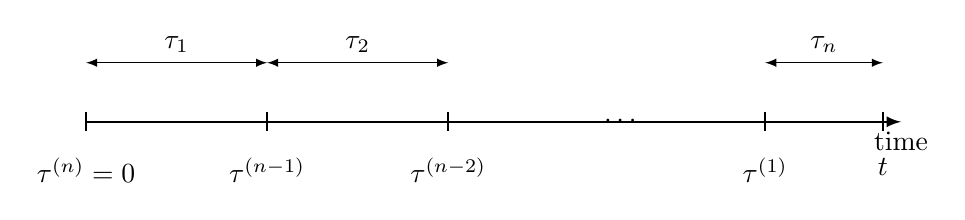
\begin{tikzpicture}[x=1.15cm,y=1cm,>=latex]
		\draw[->,thick] (0,0) -- (9,0) node[below] {time};

		% Absolute times (ticks): time-ordered interaction times plus the observation time t
		\draw[thick] (0,0.12) -- (0,-0.12) node[below=6pt] {$\tau^{(n)}=0$};
		\draw[thick] (2,0.12) -- (2,-0.12) node[below=6pt] {$\tau^{(n-1)}$};
		\draw[thick] (4,0.12) -- (4,-0.12) node[below=6pt] {$\tau^{(n-2)}$};
		\node at (5.9,0) {$\cdots$};
		\draw[thick] (7.5,0.12) -- (7.5,-0.12) node[below=6pt] {$\tau^{(1)}$};
		\draw[thick] (8.8,0.12) -- (8.8,-0.12) node[below=6pt] {$t$};

		% Delay intervals (double arrows): \tau_1, \tau_2, ..., \tau_n
		\draw[<->] (0,0.75) -- (2,0.75) node[midway,above] {$\tau_1$};
		\draw[<->] (2,0.75) -- (4,0.75) node[midway,above] {$\tau_2$};
		\draw[<->] (7.5,0.75) -- (8.8,0.75) node[midway,above] {$\tau_n$};
	\end{tikzpicture}
	\caption{Time variables in this appendix: $\tau^{(j)}$ denote absolute interaction times, while $\tau_j$ denote the nonnegative delay intervals between successive events.}
	\label{fig:app_time_variables_absolute_vs_intervals}
\end{figure}
Substituting the change of variables \autoref{eq:app_change_of_variables} into \autoref{eq:app_Pn_explicit} and assuming the system starts in equilibrium $\hat{\rho}_S(t_0)=\hat{\rho}_{\mathrm{eq}}$ at $t_0\to -\infty$, the initial evolution becomes trivial since $\mathcal{U}_0(t)[\hat{\rho}_{\mathrm{eq}}]=\hat{\rho}_{\mathrm{eq}}$ for all $t$.  The $n$-th order polarization then takes the standard operationally useful form:
\begin{equation}
	\boldsymbol{P}^{(n)}(t)
	= \int_{0}^{\infty}\!\mathrm{d}\tau_n\cdots\int_{0}^{\infty}\!\mathrm{d}\tau_1\,
	\boldsymbol{S}^{(n)}(\tau_n,\ldots,\tau_1)
	E(t-\tau_n)\,E(t-\tau_n-\tau_{n-1})\cdots E\Bigl(t-\sum_{k=1}^{n}\tau_k\Bigr),
	\label{eq:app_Pn_convolution}
\end{equation}
where the \emph{response function} $\boldsymbol{S}^{(n)}$ is defined as follows. Expanding the product of commutators in \autoref{eq:app_Pn_explicit} under the delay transformation and taking the limit $t_0\to-\infty$, the contribution that is independent of the field shape is isolated. This intrinsic material response is:
\begin{equation}
	\boldsymbol{S}^{(n)}(\tau_n,\ldots,\tau_1)
	\equiv (\mathrm{i})^n\,\mathrm{Tr}\Bigl\{\hat{\boldsymbol{\mu}}\,\mathcal{U}_0(\tau_n)\,\mathcal{V}\,\mathcal{U}_0(\tau_{n-1})\,\mathcal{V}\cdots\mathcal{V}\,\mathcal{U}_0(\tau_1)\,\mathcal{V}[\hat{\rho}_{\mathrm{eq}}]\Bigr\}.
	\label{eq:app_Sn_def}
\end{equation}
Equation \autoref{eq:app_Sn_def} defines the (causal) \emph{response function}: $\boldsymbol{S}^{(n)}(\tau_n,\ldots,\tau_1)$ describes the intrinsic material response to $n$ successive light--matter interactions separated by the delay intervals $(\tau_n,\ldots,\tau_1)$. Crucially, $\boldsymbol{S}^{(n)}$ depends only on the field-free dynamics $\mathcal{U}_0$ and the dipole operator (through $\mathcal{V}$), and is completely independent of the particular pulse shapes or envelope functions $E(t)$. This is what makes response functions a fundamental and universal characterization of nonlinear material properties.
The nested-commutator structure that emerges from expanding the product in \autoref{eq:app_Sn_def} is essential for understanding nonlinear spectroscopy. Since each interaction produces a left and a right action on the density operator as shown in \autoref{eq:app_V_commutator_expanded}. Expanding the product of $n$ commutators therefore generates $2^n$ distinct Liouville-space contributions or ``pathways'' before additional physical selections (e.g., rotating-wave approximation, phase matching/phase cycling) restrict the subset that contributes to a given measured signal. These pathways are naturally represented by double-sided Feynman diagrams, where the two branches represent the ket and bra evolution and each field interaction is drawn as an arrow acting from the left or from the right~\cite{mukamel1995principlesnonlinearoptical}.

A final important point: while the Dyson series (\autoref{eq:app_dyson}) itself is strictly time ordered with $\tau_1>\tau_2>\cdots>\tau_n$, in a real experiment the three pulses can arrive in any order. Different pulse orderings correspond to different time-ordered contributions to $\boldsymbol{P}^{(n)}$. The experimentally measured total response is obtained by summing the relevant orderings for the chosen pulse sequence.

Two points are emphasized. First, causality is explicit: $\boldsymbol{S}^{(n)}$ is only needed for nonnegative delays, and the fields are evaluated at times earlier than $t$. Second, $\boldsymbol{S}^{(n)}$ depends only on field-free dynamics and the dipole operator. It is independent of the particular pulse shapes.

\section{Tensor structure and polarization components}
\label{app:sec:tensorial_structure}

If one does not fix a single polarization direction, the response becomes a rank-$(n{+}1)$ tensor. Introduce component dipole superoperators
\begin{equation*}
	\mathcal{V}_\beta[\hat{A}] \equiv [\hat{\mu}_\beta,\hat{A}],\qquad \beta\in\{x,y,z\},
\end{equation*}
and define
\begin{equation*}
	S^{(n)}_{\alpha\beta_1\cdots\beta_n}(\tau_n,\ldots,\tau_1)
	= (\mathrm{i})^n\,\mathrm{Tr}\Bigl\{\hat{\mu}_\alpha\,\mathcal{U}_0(\tau_n)\,\mathcal{V}_{\beta_n}\,\mathcal{U}_0(\tau_{n-1})\,\mathcal{V}_{\beta_{n-1}}\cdots\mathcal{U}_0(\tau_1)\,\mathcal{V}_{\beta_1}[\hat{\rho}_{\mathrm{eq}}]\Bigr\}.
\end{equation*}
Then $P^{(n)}_\alpha(t)$ is obtained by contracting this tensor with the field components $E_{\beta}(t)$. Choosing a fixed unit polarization $\mathbf e$ and writing $E_\beta(t)=e_\beta E(t)$ reduces the tensorial form back to \autoref{eq:app_Pn_convolution}.



\section{Explicit linear and third-order response}
\label{app:sec:linear_and_third_order_response}

The linear (first-order) response is briefly discussed as it represents the simplest case of light-matter interaction, illustrating fundamental absorption and dispersion processes. The third-order response is examined in detail, as it forms the foundation for two-dimensional Fourier transform (2DFT) spectroscopy.

\subsection{Linear response}
With $n=1$, the first-order (linear) polarization is
\begin{equation*}
	\boldsymbol{P}^{(1)}(t)
	= \int_{0}^{\infty}\!\mathrm{d}\tau_1\,\boldsymbol{S}^{(1)}(\tau_1)\,E(t-\tau_1),
\end{equation*}
where the linear response function $\boldsymbol{S}^{(1)}(\tau_1)$ from \autoref{eq:app_Sn_def} with $n=1$ is
\begin{equation*}
	\boldsymbol{S}^{(1)}(\tau_1)
	= \mathrm{i}\,\mathrm{Tr}\bigl\{\hat{\boldsymbol{\mu}}\,\mathcal{U}_0(\tau_1)\,\mathcal{V}[\hat{\rho}_{\mathrm{eq}}]\bigr\}.
\end{equation*}
This linear response describes absorption and dispersion of the incident field.

\subsection{Third-order response}
For the third-order term central to 2D spectroscopy, $n=3$ is used in \autoref{eq:app_Pn_convolution}:
\begin{equation}
	\boldsymbol{P}^{(3)}(t)
	= \int_{0}^{\infty}\!\mathrm{d}\tau_3\int_{0}^{\infty}\!\mathrm{d}\tau_2\int_{0}^{\infty}\!\mathrm{d}\tau_1\,\boldsymbol{S}^{(3)}(\tau_3,\tau_2,\tau_1)
	\,E(t-\tau_3)\,E(t-\tau_3-\tau_2)\,E(t-\tau_3-\tau_2-\tau_1),
	\label{eq:app_P3_convolution}
\end{equation}
where the third-order response function $\boldsymbol{S}^{(3)}(\tau_3,\tau_2,\tau_1)$ from \autoref{eq:app_Sn_def} with $n=3$ is
\begin{equation}
	\boldsymbol{S}^{(3)}(\tau_3,\tau_2,\tau_1)
	= (\mathrm{i})^3\,\mathrm{Tr}\Bigl\{\hat{\boldsymbol{\mu}}\,\mathcal{U}_0(\tau_3)\,\mathcal{V}\,\mathcal{U}_0(\tau_2)\,\mathcal{V}\,\mathcal{U}_0(\tau_1)\,\mathcal{V}[\hat{\rho}_{\mathrm{eq}}]\Bigr\}.
	\label{eq:app_S3_def}
\end{equation}
This third-order response captures all two-quantum coherence and collective effects in the material. In a multi-pulse 2D experiment, the incident field is decomposed into three pulse envelopes: $E(t)=E_1(t)+E_2(t)+E_3(t)$. When substituted into \autoref{eq:app_P3_convolution}, this generates many terms. Experimentally, the desired third-order signal (e.g., the rephasing pathway) is isolated by phase matching or phase cycling. The response function \autoref{eq:app_S3_def} provides the causal kernel underlying that selection~\cite{hammzanni2011conceptsmethods2d}.


\textbf{Remark on frequency-domain.}
For completeness, the frequency domain is sometimes convenient. After decomposing each incident field into positive and negative frequency components (complex fields and their conjugates), the convolution in \autoref{eq:app_P3_convolution} transforms into an algebraic product in frequency space. A compact bookkeeping form for third-order mixing is
\begin{equation*}
	P_i^{(3)}(t)
	=
	\varepsilon_0
	\sum_{jkl}
	\sum_{\sigma_1,\sigma_2,\sigma_3=\pm 1}
	\chi^{(3)}_{ijkl}\big(-\omega_S;\sigma_1\omega_1,\sigma_2\omega_2,\sigma_3\omega_3\big)
	\,E_{1,j}^{(\sigma_1)}E_{2,k}^{(\sigma_2)}E_{3,l}^{(\sigma_3)}\,e^{-i\omega_S t},
\end{equation*}
with $\omega_S=\sigma_1\omega_1+\sigma_2\omega_2+\sigma_3\omega_3$. This form shows how the third-order susceptibility tensor $\chi^{(3)}$ governs the frequency mixing. Fixing all field polarization directions reduces this general tensorial expression to a scalar that matches expressions used throughout the main text.


\medskip
It is worth pausing to note what has been accomplished. Starting from the microscopic equation of motion (\autoref{eq:app_master_equation_with_field}), invoking the Dyson series to generate a perturbative expansion, transforming to experimentally natural time intervals, and assuming equilibrium initial conditions, an explicit and causal expression for $\boldsymbol{P}^{(n)}(t)$ has been derived as a convolution of a system-dependent response function with the incident fields. In nonlinear spectroscopy, this is not merely a formal mathematical result: each term of fixed order corresponds to a real, experimentally isolable physical process (selectable by phase matching or phase cycling), and the response function $\boldsymbol{S}^{(n)}$ provides the system-specific, causal "memory kernel" through which the incident fields probe the material.

This appendix stops here. Detection models (homodyne/heterodyne) and the construction of 2D spectra from the phase-selected time-domain signals are discussed in \autoref{chapter_spectroscopy}, \autoref{sec:2D_construction_formal}.

